\section{PPM deviates from AC}
\begin{frame}
    \frametitle{114e/485o}
    \begin{figure}
        \centering
        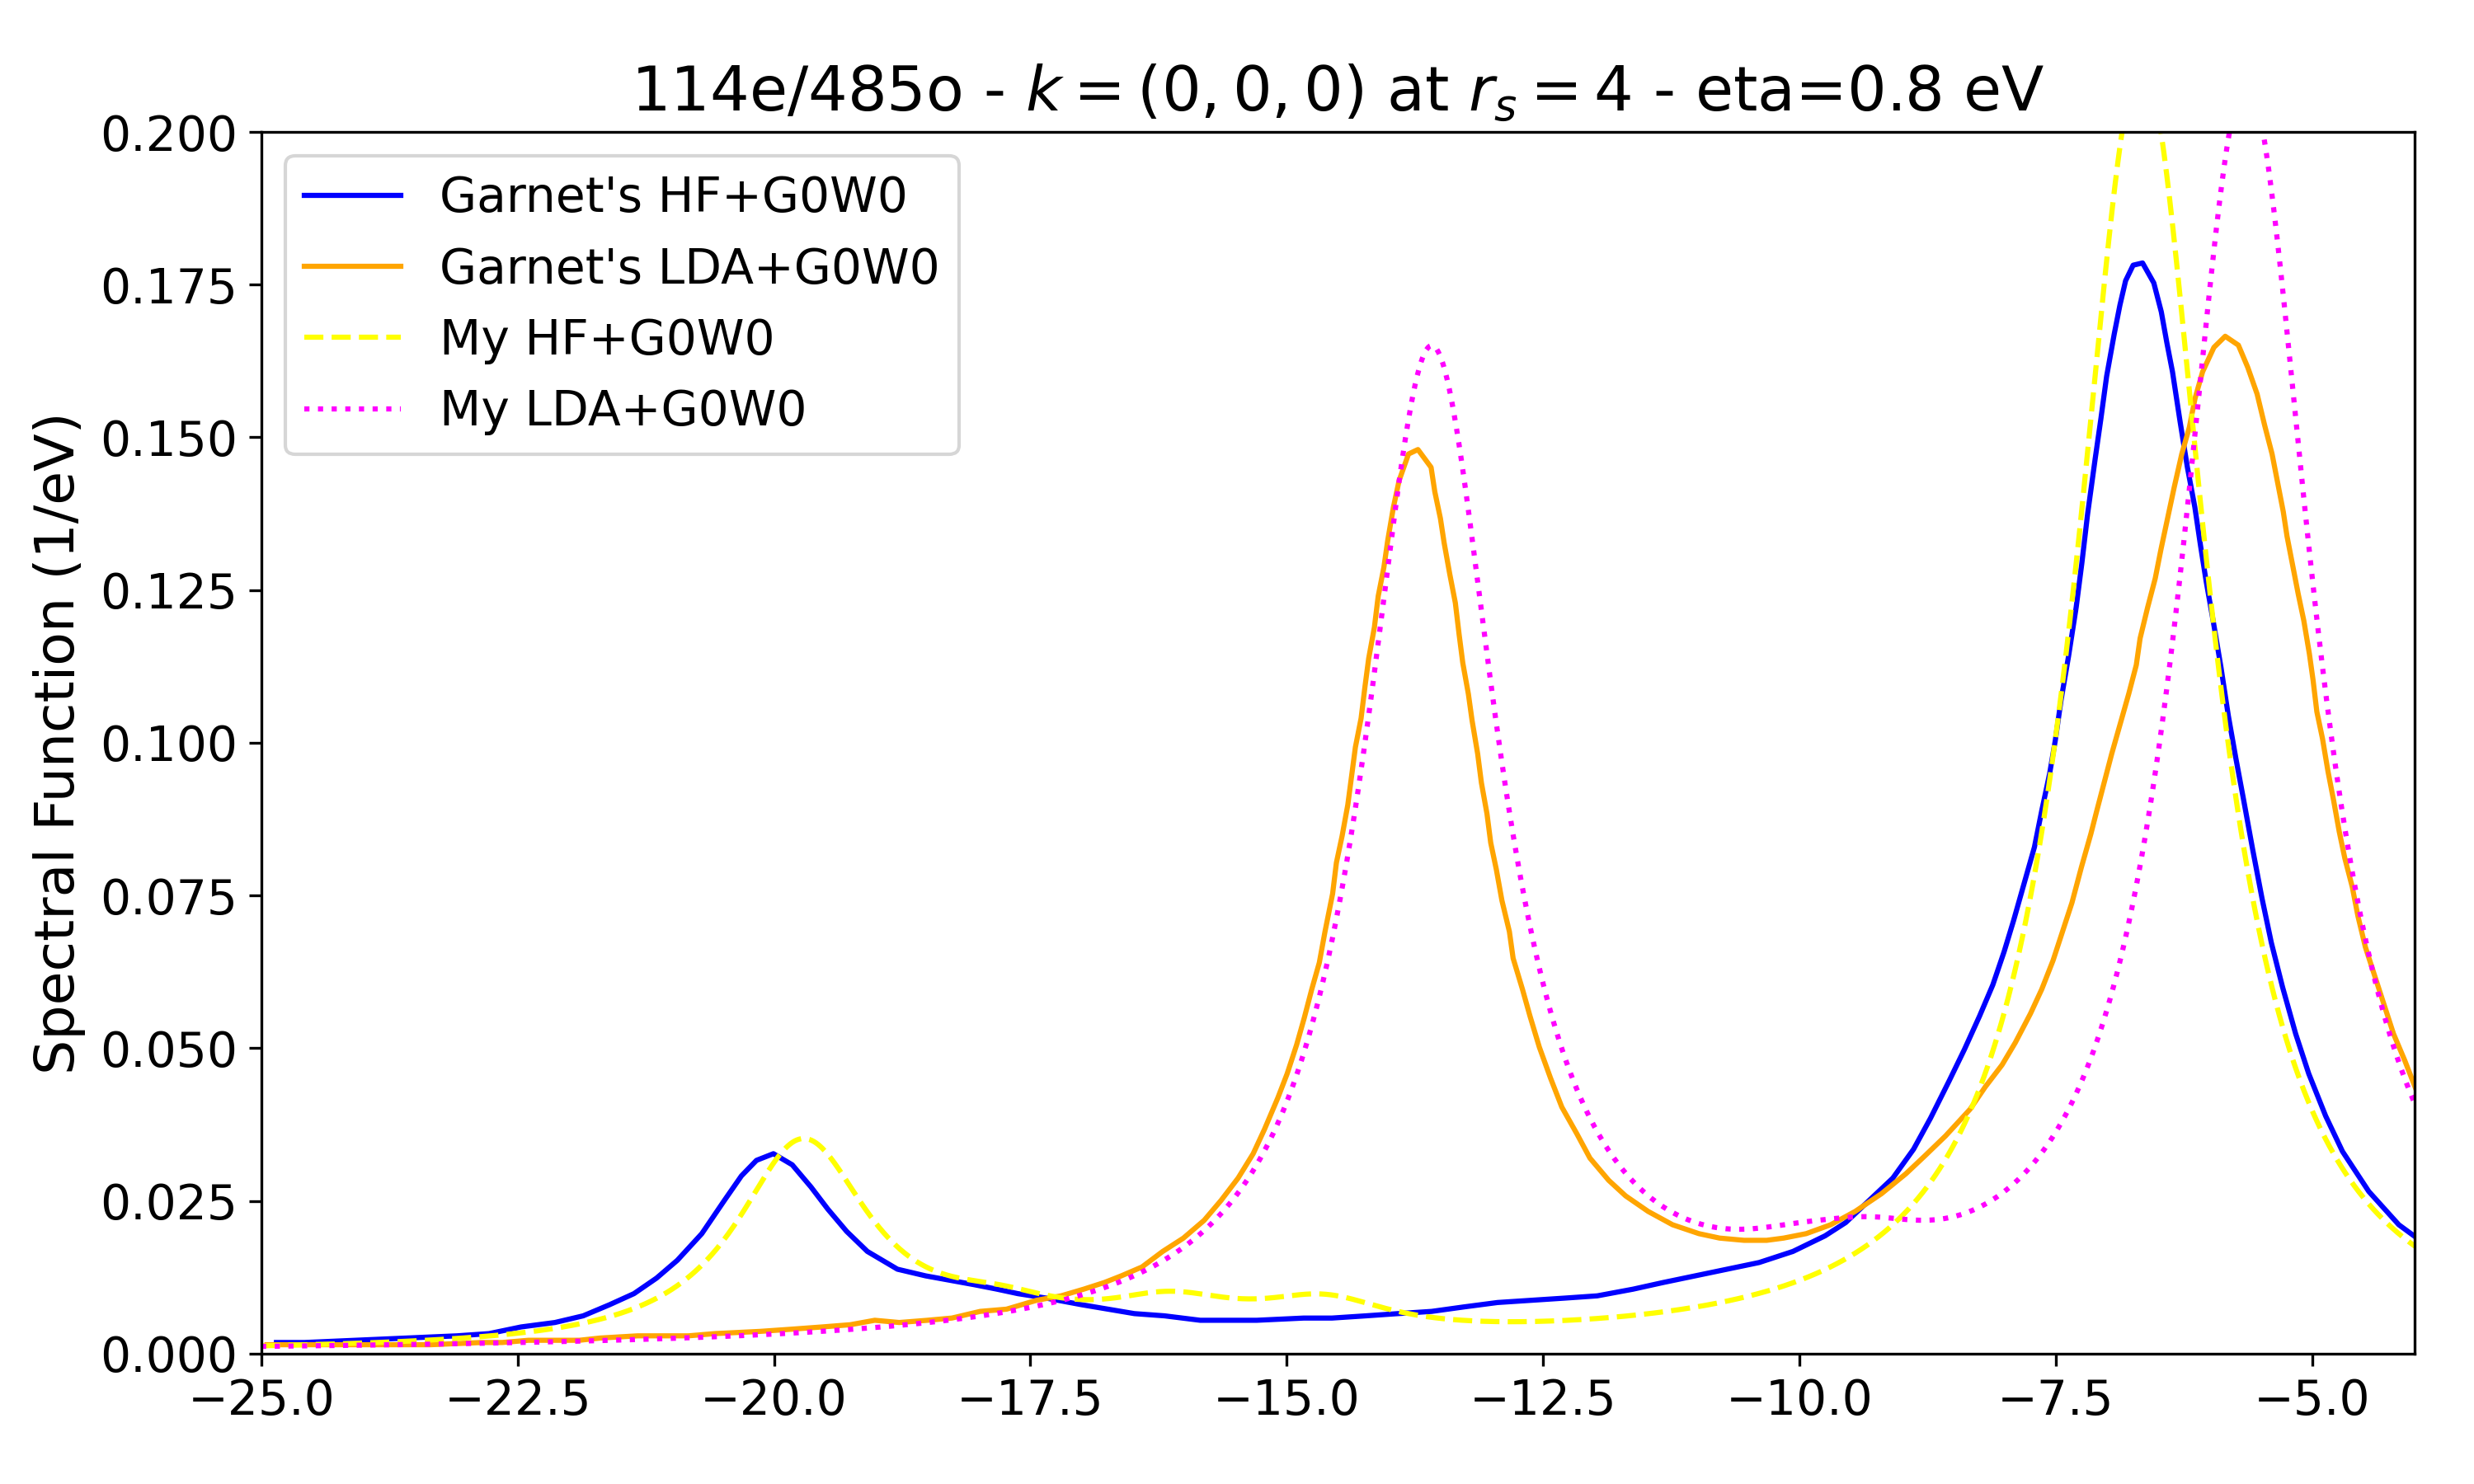
\includegraphics[width=\textwidth]{figs/6-12/refpgw.png}
    \end{figure}
\end{frame}
\begin{frame}
    \frametitle{14e/57o}
    \begin{figure}
        \centering
        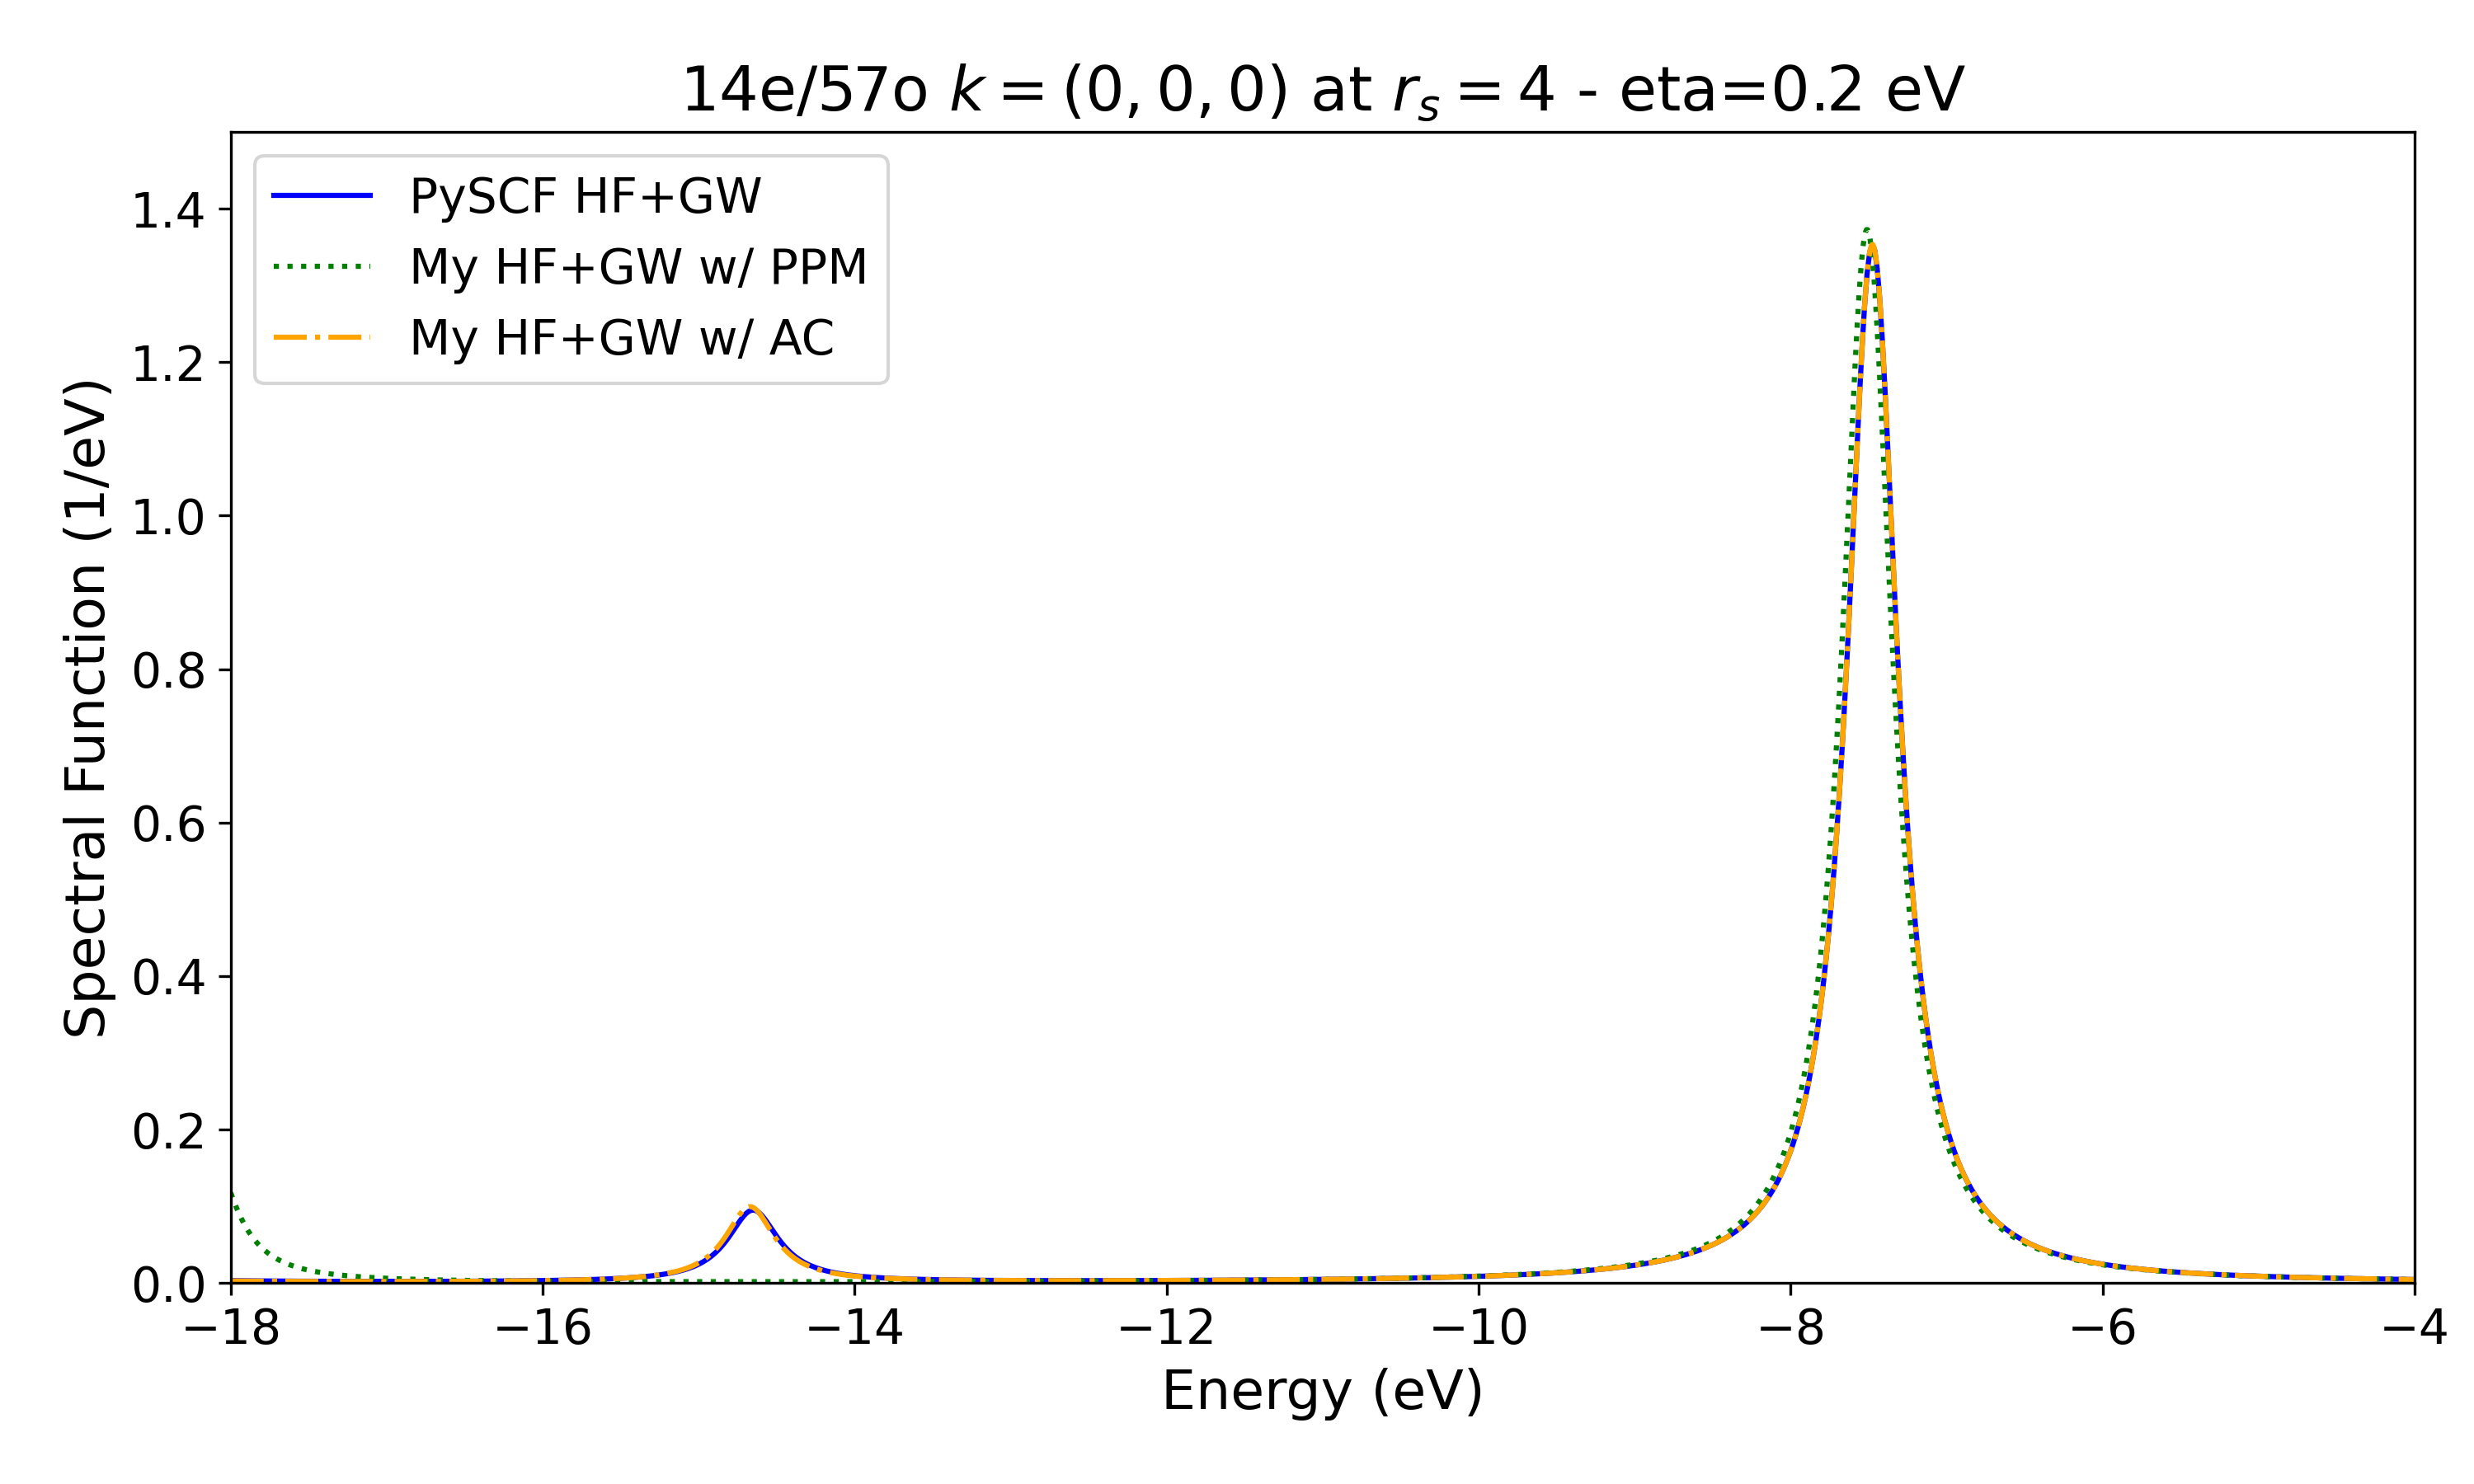
\includegraphics[width=\textwidth]{figs/6-12/gw_14e57o.png}
    \end{figure}
\end{frame}
\section{Why I don't think AC is the right answer}
\begin{frame}
    \frametitle{Theory}
\begin{align}
    \Sigma_{n n^{\prime}}^c(\mathbf{k}, i \omega)&= -\frac{1}{\pi N_{\mathbf{k}}} \sum_{m \mathbf{q}} \int_0^{\infty} d \omega^{\prime} \frac{i \omega+\epsilon_F-\epsilon_{m \mathbf{k}-\mathbf{q}}}{\left(i \omega+\epsilon_F-\epsilon_{m \mathbf{k}-\mathbf{q}}\right)^2+\omega^{\prime 2}}\\
&\times  \sum_{P Q} v_P^{n m}\left[\left[\mathbf{I}-\mathbf{\Pi}\left(\mathbf{q}, i \omega^{\prime}\right)\right]_{P Q}^{-1}-\delta_{P Q}\right] v_Q^{m n^{\prime}}
\end{align}\pause
with the polarizability given by
\begin{equation}
\boldsymbol{\Pi}_{P Q}\left(\mathbf{q}, i \omega^{\prime}\right)=\frac{2}{N_{\mathbf{k}}} \sum_{\mathbf{k}} \sum_i^{\text {occ }} \sum_a^{\text {vir }} v_P^{i a} \frac{\epsilon_{i \mathbf{k}}-\epsilon_{a \mathbf{k}-\mathbf{q}}}{\omega^{\prime 2}+\left(\epsilon_{i \mathbf{k}}-\epsilon_{a \mathbf{k}-\mathbf{q}}\right)^2} v_Q^{a i}.
\end{equation}\pause
Then form Pade approximants as
\begin{equation}
    \Sigma_{n n^{\prime}}(\mathbf{k}, \mathbf{z})=\frac{a_0+a_1 \cdot \mathbf{z}+\ldots+a_{(N-1) / 2} \cdot z^{(N-1) / 2}}{1+b_1 \cdot \mathbf{z}+\ldots+b_{N / 2} \cdot z^{N / 2}}
\end{equation}\pause
and then analytically continue to the real axis.
\end{frame}
\begin{frame}
    \frametitle{38e/123o example}
    \begin{figure}
        \centering
        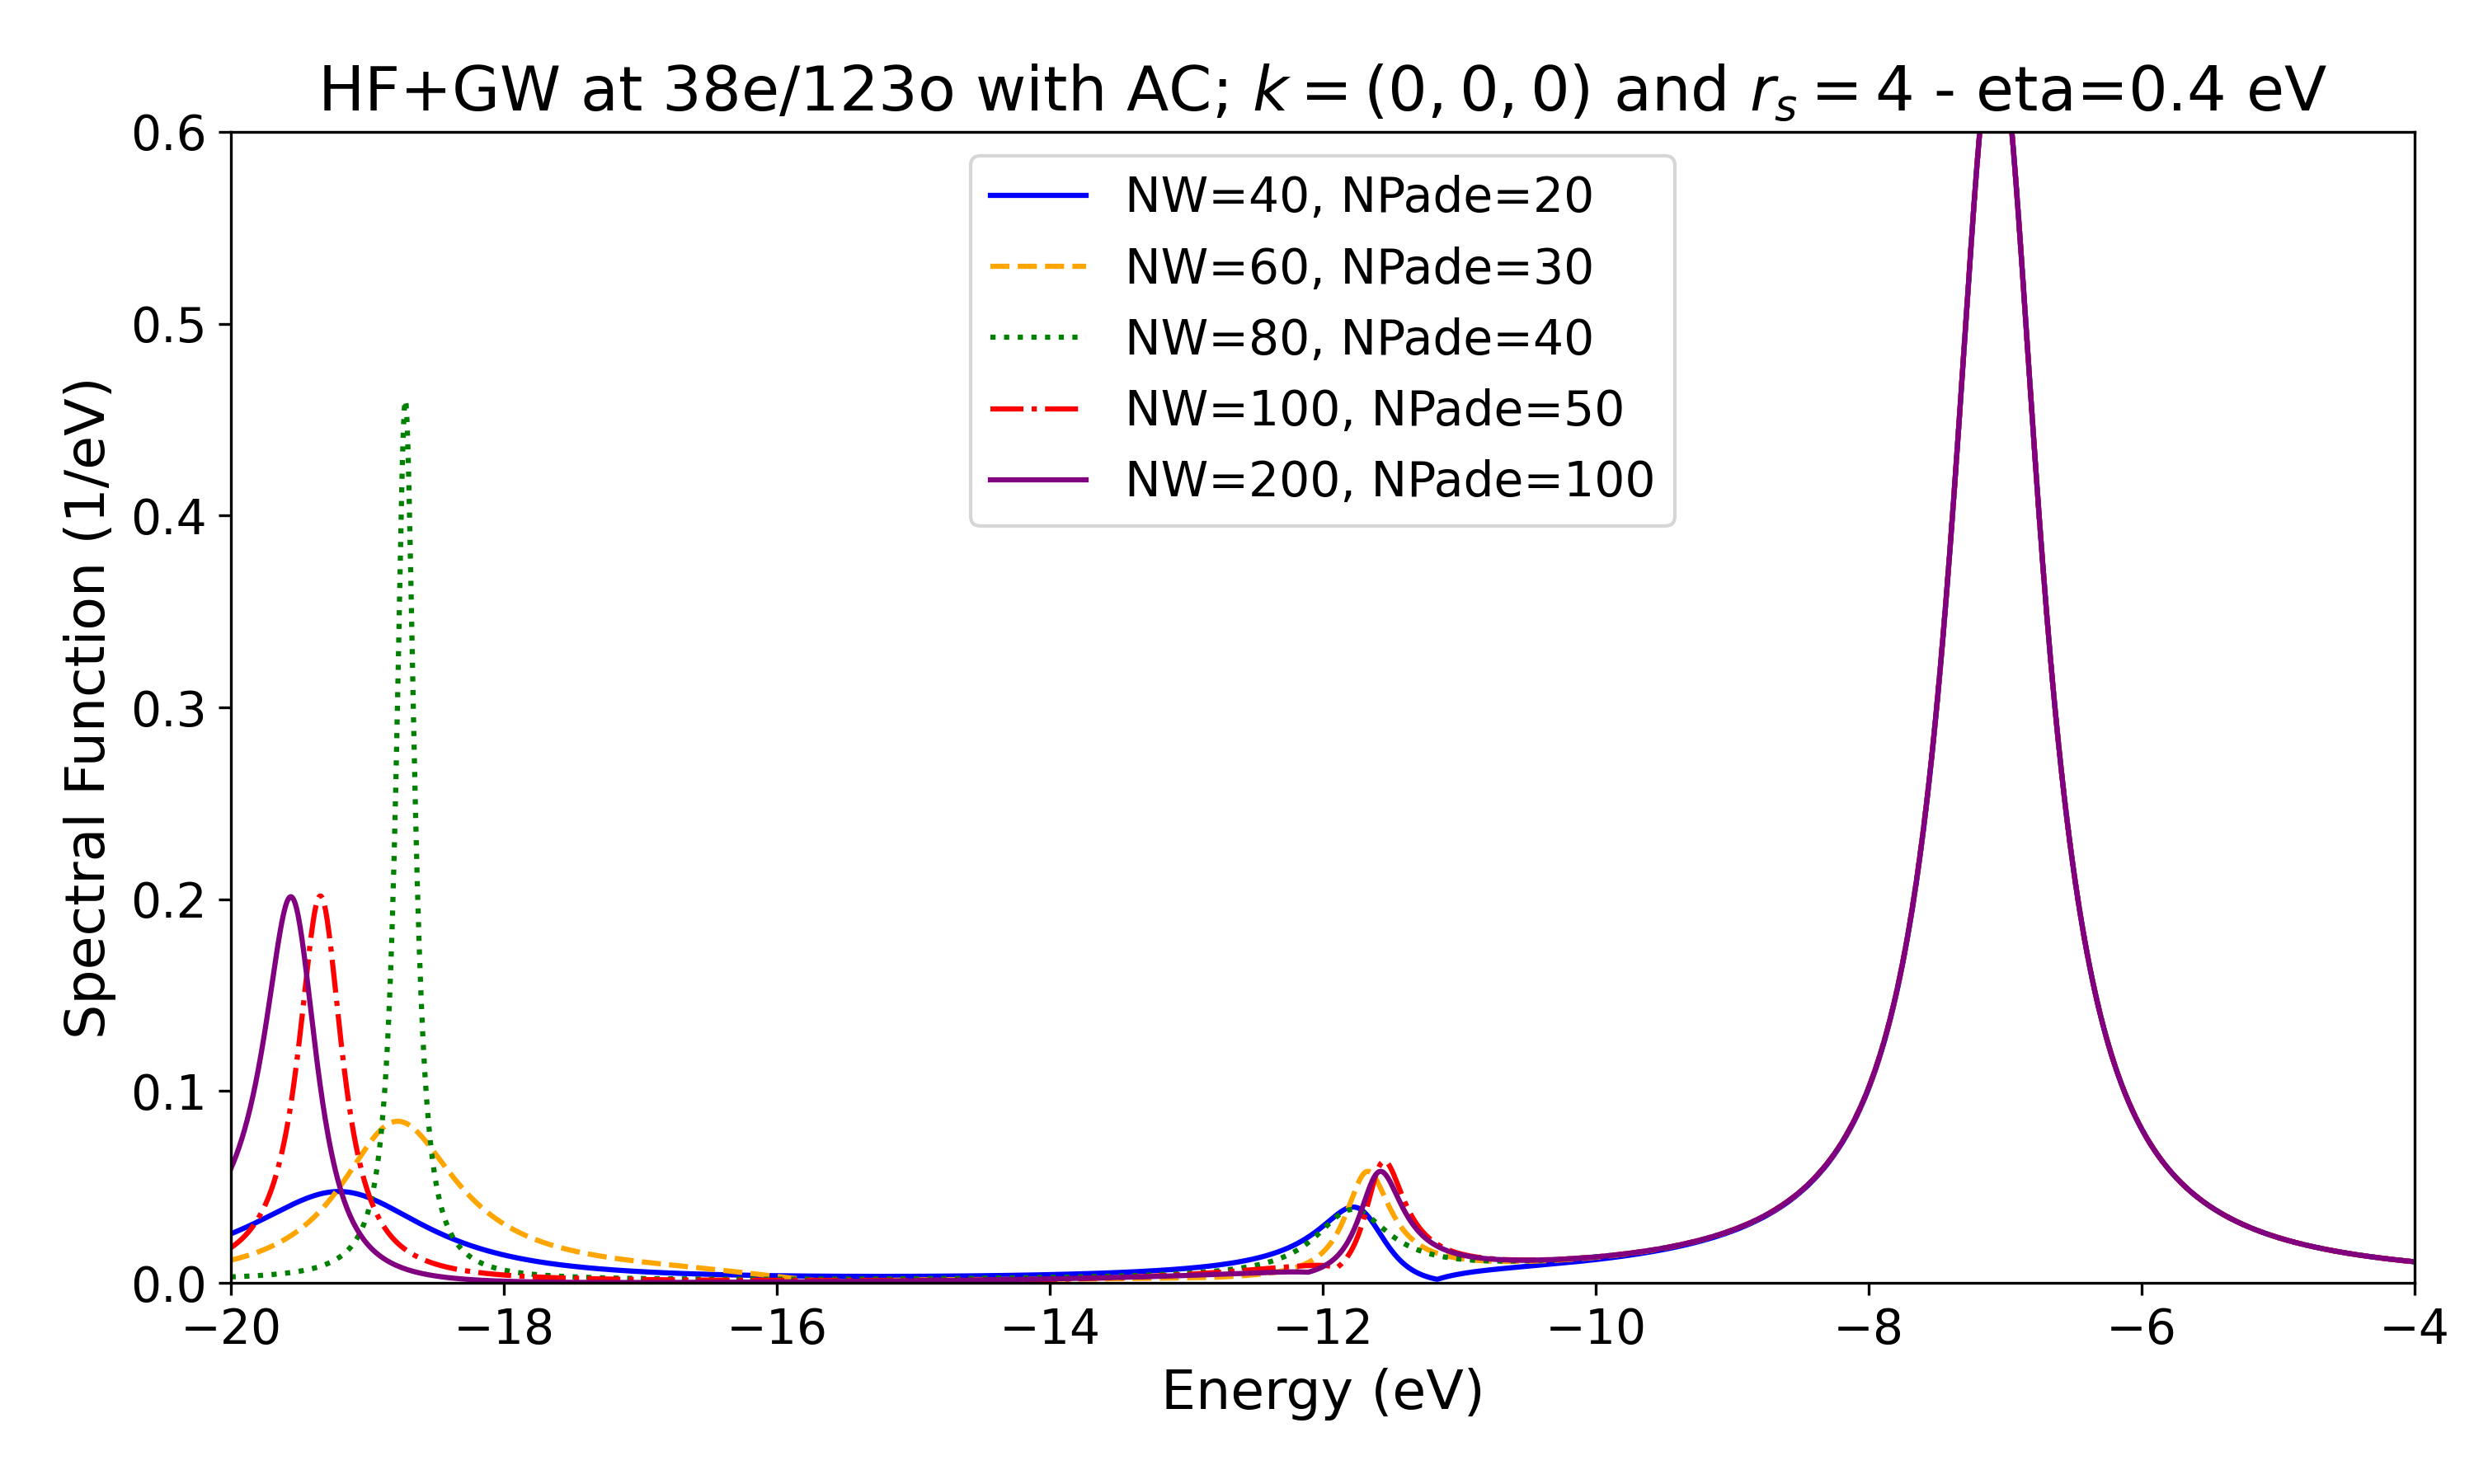
\includegraphics[width=\textwidth]{figs/6-12/gw_38e123o_ac.png}
    \end{figure}
\end{frame}
\begin{frame}
    \frametitle{Why using AC would be problematic for us}
\begin{itemize}
    \item Known to be numerically unstable for QP energies of deep core states. \pause
    \item Getting satellite features even more difficult. \pause
    \item Looked good for 14e/19o because this wasn't a true core state? \pause
    \item Need to run CD alongside AC and PPM for 114e/485o to verify this. 
\end{itemize}
\end{frame}
\begin{frame}
    \frametitle{Contour deformation for 14e/19o}
    \begin{figure}
        \centering
        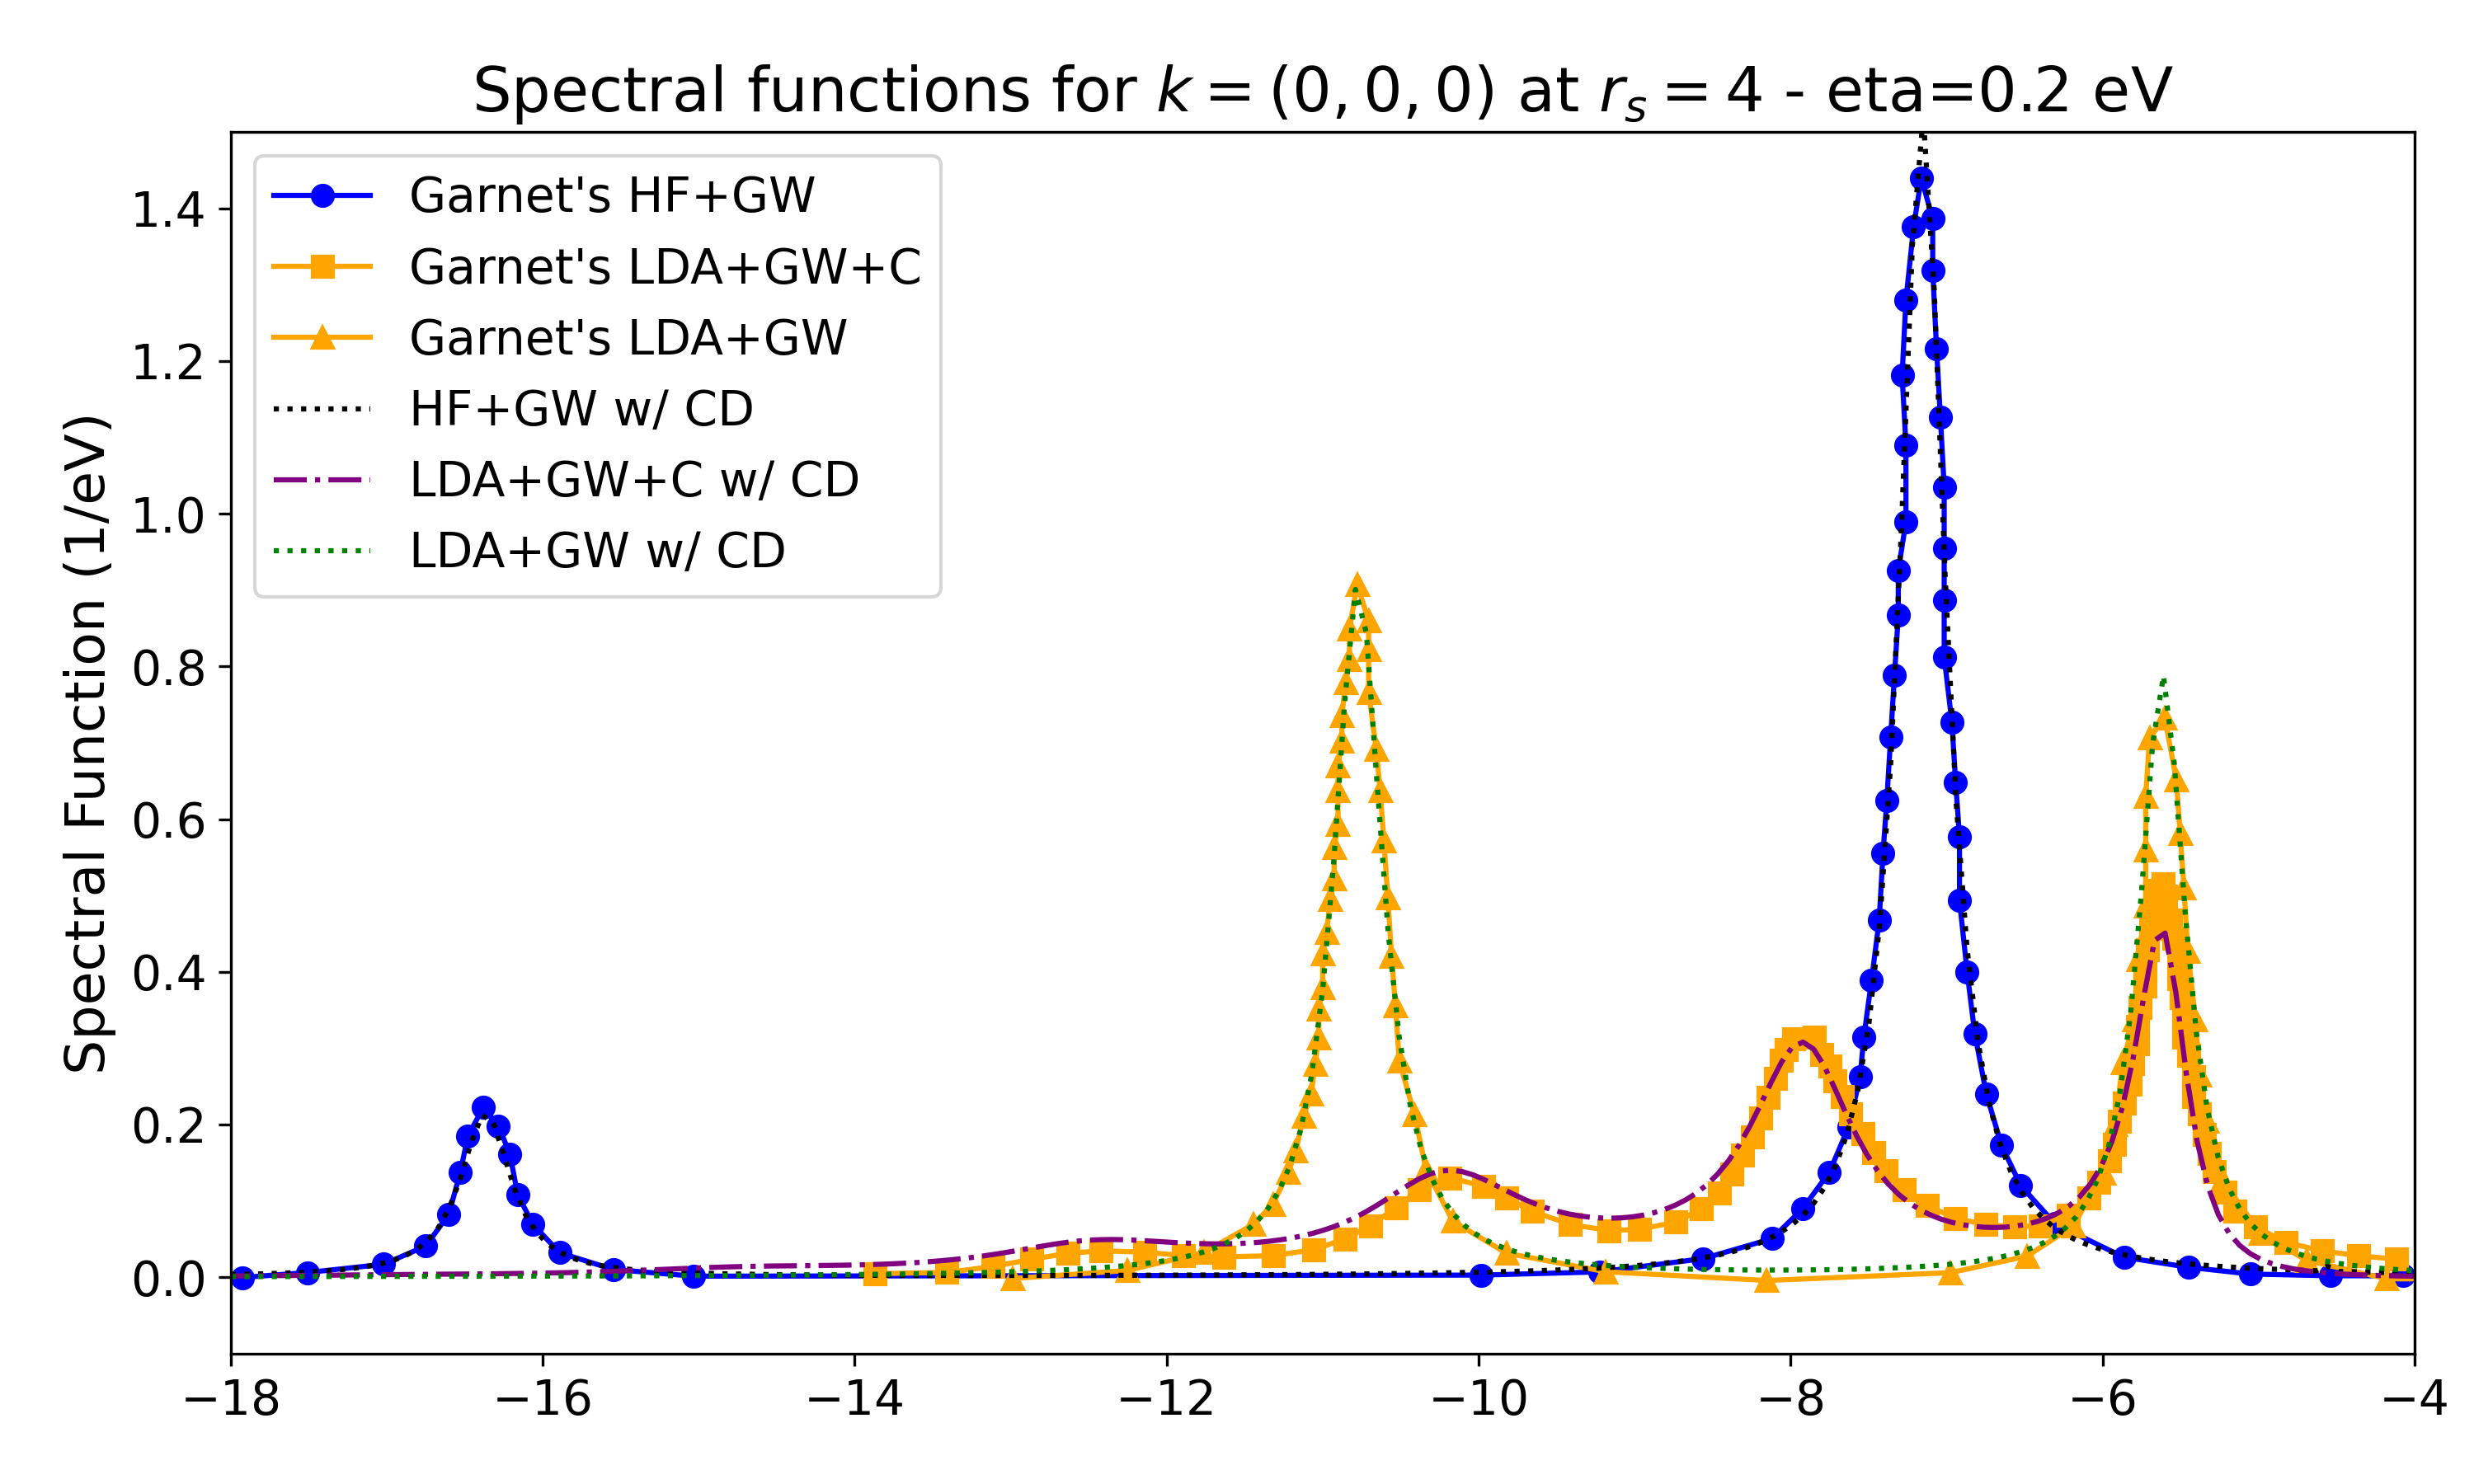
\includegraphics[width=\textwidth]{figs/6-12/gw_cd_verification.png}
    \end{figure}
\end{frame}
\section{Open questions}
\begin{frame}
    \frametitle{Open questions}
\begin{itemize}
    \item Should I spend time figuring out the bug in my PPM code? \pause
    \item Bad idea to run the $O(N^6)$ Casida diagonalization for 114e/485o?
\end{itemize}
\end{frame}
